\chapter{Overview of Testing Techniques}
\label{cha:overview-of-testing}

(Summary of chapter)

\section{Definition of Testing}
\label{sec:definition-of-testing}

Testing \cite{myers-1979}

Other basic definitions

\subsubsection{Test oracle}

\begin{figure}[ht]
    \centering
    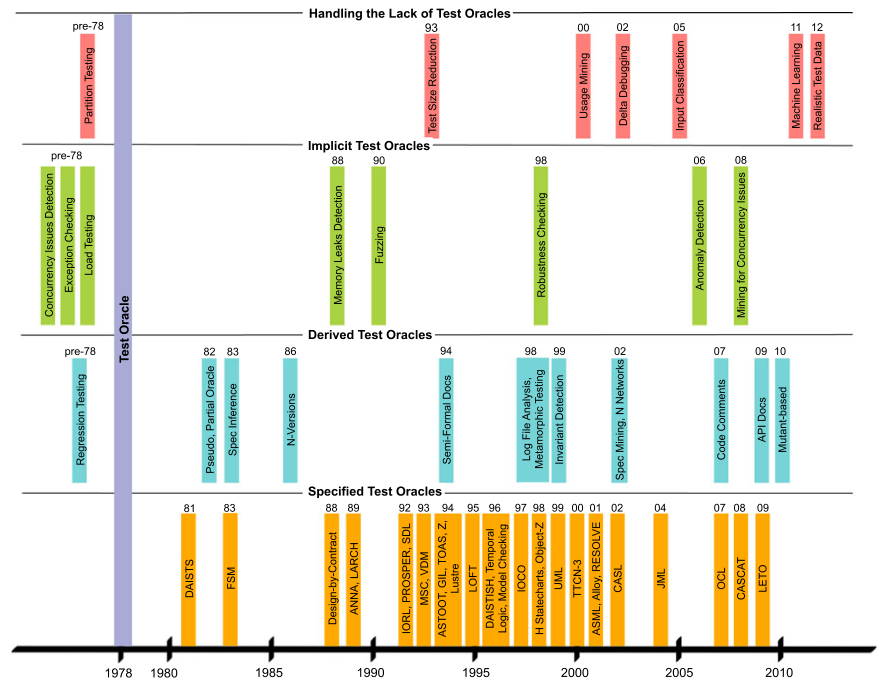
\includegraphics[width=0.9\textwidth]{figures/oracle-survey-techniques}
    \caption{Oracle techniques and concepts \cite{oracle-survey}}
    \label{fig:overview-of-testing:oracle-survey-techniques}
    \end{figure}

\section{Testing Process}
\label{sec:testing-process}

\begin{enumerate}
    \item Planning and Control
    \item Analysis and Design
    \item Implementation and Execution
    \item Evaluating Exit Criteria and Reporting    
    \item Test Closure
\end{enumerate}

Test generation will be a different chapter \cite{Anand13}.


\section{Hungarian terms}

\begin{table}[ht]
    \centering
    \small
    \caption{Hungarian terms for overview of testing chapter}
    \begin{tabular}{ll}
        \toprule
        \textbf{English} & \textbf{Hungarian} \\
        \midrule
        acceptance test & átvételi teszt \\
        exhaustive testing & kimerítő tesztelés \\
        expected outcome & elvárt eredmény \\
        exploratory testing & felderítő tesztelés \\
        fail & sikertelen teszt (bukás) \\
        oracle & orákulum \\
        pass & sikeres teszt \\
        test case & teszteset \\
        test basis & tesztbázis \\
        test design & (műszaki) teszttervezés \\
        test object & teszt tárgya \\
        test objective & tesztcél \\
        test suite & tesztkészlet \\
        \bottomrule
    \end{tabular}
    \label{tab:overview:hungarian-terms-testing-overview}
\end{table} 